\chapter{Evaluation}
\label{ch:evaluation}
This chapter presents the evaluation of the implemented WebCrowd platform through a series of experiments designed to address the research questions defined in \autoref{subsec:into:objectives:questions}. These three research questions focus on WebCrowds computational capabilities when handling complex parallelizable tasks, its dynamic viability in managing fluctuating worker participation, and its ability to support heterogeneous devices as workers. Each of the following sections in this chapter corresponds to one of the research questions and presents the experimental setup, the expected outcome, and a analysis of these results.

The experiments of the evaluation utilize the implemented visualization of the Mandelbrot set, described in \autoref{sec:implementation:benchmark}, as a benchmark job. This benchmark job represents a computationally intensive test case, which can be used to demonstrate and test WebCrowd's capabilities. Each task of this benchmark job coveres a unique 1500x1500 area of the Mandelbrot set and all generated \ac{PNG} files have the same resolution. However, the computation time varies significantly among each of these tasks. According to the Mandelbrot function in (\ref{equ:mandelbrot}) require complex numberers that are part of the Mandelbrot set more iterations of the calculation than complex numbers that are not part of the Mandelbrot set. Therefore depends the execution time of a task on the amount of calculated points that belong to the Mandelbrot set.

Additionally, \autoref{sec:evaluation:languages} compares the performance of the various in WebCrowd implemented WebAssembly environments, each supporting the execution of source code from different programming languages compiled to a WebAssembly binary.

\section{Computational Capability}
\label{sec:evaluation:computation}
\textbf{Is WebCrowd capable of successfully solving large, parallelizable problems?} 
\newline
The objective of the following experiment is to evaluate WebCrowd's ability to successfully execute computationally intensive, parallelizable tasks across a distributed network of volunteer workers. This empirical experiment compares the total execution time between distributed computation across multiple workers and native execution on a single computer.

\subsection{Experimental Setup}
The batch size of the benchmark job was set to 101. Therfore, only a singel batch is generated and processed during all experiments and the job progress is only persisted once upon completion of all 101 tasks.

At first the benchmark job was computed on the system specified in \autoref{app:system:server} in a native Go environment using the source code of \autoref{app:code:mandelbrot3}. The resulting computation time serves as a baseline for the following experiments, because this system is later also used to host the WebCrowd platform. Since this system is already required to serve WebCrowd in the first place, the following experiments additionally investigate whether distributing the workload to external clients provides a performance advantage compared to utilizing the existing host system for computation. Throughout the experiments, all workers maintained available and executed only the WebCrowd browser process. The benchmark job was evaluated across the following six distinct scenarios:
\begin{itemize}
    \item Two homogeneous and independent smartphones with the harware specified in \autoref{app:system:phone} as workers, executing the client page in a Apple Safari 18.1 \cite{evaluation:safari} browser
    \item Three homogeneous and independent smartphones with the harware specified in \autoref{app:system:phone} as workers, executing the client page in a Apple Safari 18.1 \cite{evaluation:safari} browser
    \item Three parallel Mozilla Firefox 132.0 \cite{background:firefox} browser taps of the client page on a single laptop, specified in \autoref{app:system:mymachine}
    \item Three parallel Microsoft Edge 131.0.0.0 \cite{evaluation:edge} browser taps of the client page on the same \acs{PC}, specified in \autoref{app:system:mypc}
    \item 16 homogeneous and independent single-board computers with the harware specified in \autoref{app:system:pi} as workers, each executing the client page in a headless Mozilla Firefox 133.0 \cite{background:firefox2} browser
    \item 32 homogeneous and independent single-board computers with the harware specified in \autoref{app:system:pi} as workers, each executing the client page in a headless Mozilla Firefox 133.0 \cite{background:firefox2} browser
\end{itemize}

\subsection{Expectations}
It is expected that all tasks of the benchmark job will be scheduled as intended and distributed over all participating workers and each task result is successfully received by the server and saved on the server. To verify if this process was successful, each worker is monitored through the interface of the client page during the experiment and after the experiment is the implemented mandelbrot page (\autoref{sec:implementation:benchmark}) utilized to examine the generated task results.

Additinally, all experiments are carried out using the interactive dashboard page (\autoref{subsec:implementation:dashboard-page}) to start and monitor the execution of the benchmark job. It is expected that all features of this application work as intended and the job progress as well as all participating workers can be monitored in real-time.

Furthermore, based on the theoretical model presented in \autoref{sec:background:theory}, distributing the benchmark job across multiple workers should reduce the total execution time of a job when the number of workers $N$ exceeds the threshold value represented in the inequality term of \eqref{equ:transformation2}. To estimate this threshold value of $N$ for all previously listed experiment scenarios the amount of tasks $T$ was set to 101 and an Internet latency of 32 ms \cite{backend:latency} was assumed for $t_{L}$. Since the computation times $t_{Native}$ and $t_{Virtual}$ are not equal for all 101 tasks, a heavy computational task - handeling the center of the Mandelbrot set - was selected to represent these computation times. This single task has been executed and measured independently on the native Go environment on the server system as well as on the WebAssembly browser environment through the WebCrowd platform for each device participating in the experiment as worker. The computation time $t_{Native}$ of this computationally heavy task was measured to be 34.60 seconds on the server system specified in \autoref{app:system:server}. The corresponding computation time $t_{Virtual}$ of the same task was measured to be 57.53 seconds using the Apple Safari 18.1 \cite{evaluation:safari} browser on a smartphone specified in \autoref{app:system:phone}, 1 minute and 34.8 seconds using the Mozilla Firefox 132.0 \cite{background:firefox} browser on the laptop specified in \autoref{app:system:mymachine}, 1 minute and 28.2 seconds using the Microsoft Edge 131.0.0.0 \cite{evaluation:edge} browser on the \acs{PC} specified in \autoref{app:system:mypc} and a total of 7 minutes and 13.2 seconds using the headless Mozilla Firefox 133.0 \cite{background:firefox2} browser on one single-board computer specified in \autoref{app:system:pi}. With this information the amount of workers $N$ - expected to provide a performance advantage compared to the native code execution - was calculated with the inequality term of \eqref{equ:transformation2} for each scenerio:
\begin{itemize}
    \item \textbf{Smartphones:} $N > 1.7$, meaning two or more smartphones are expected to achieve a performance gain 
    \item \textbf{Laptops:} $N > 2.8$, meaning three or more laptops are expected to achieve a performance gain
    \item \textbf{PCs:} $N > 2.6$, meaning three or more \acs{PC}s are expected to achieve a performance gain
    \item \textbf{Single-board computers:} $N > 14.3$, meaning 15 or more single-board computers are expected to achieve a performance gain
\end{itemize}

\subsection{Results}
The benchmark job was successfully computed in every experiment and all features of the web application behaved as intended.
\newpage
\begin{figure}[htbp]
    \centering
    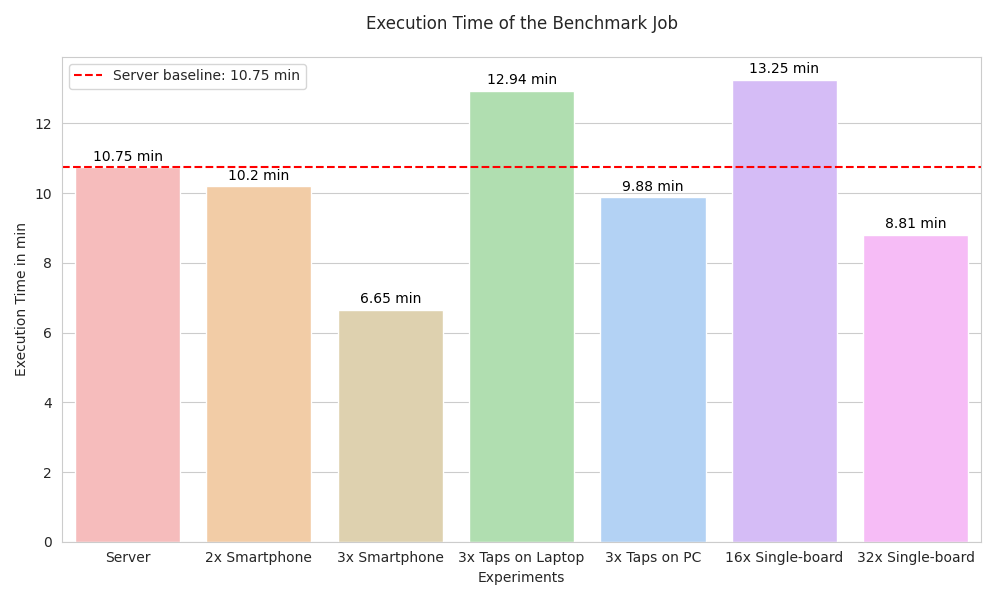
\includegraphics[width=0.95\textwidth]{gfx/figures/Evaluation_A.png}
    \caption{WebCrowd Execution Time Compared to Native Execution Time}
    \label{fig:evaluation:experiment-A}
\end{figure}
~\\
\autoref{fig:evaluation:experiment-A} compares the measured execution times of the different experiments to the baseline time of the server. The native execution on the server system completed all 101 tasks in an average execution time $t_{ExSeq}$ of 10 minutes and 45 seconds across three runs. Distributing the benchmark job across the two smartphone workers resulted in a total execution time $t_{ExDist}$ of 10 minutes and 12 seconds, and therfore faster than the baseline as predicted. With three smartphone workers, the execution time further decreased to 6 minutes and 39 seconds, representing a performance improvement of 38\% compared to the native execution on the server. 

Distributing the benchmark job across three browser taps on the laptop took 12 minutes and 56.4 seconds to complete the total workload. This approach did not achieve a performance gain compared to the native code execution on the server. However, distributing the benchmark job across three browser taps on the \acs{PC} complete the total workload in only 9 minutes and 52.8 seconds and therfore faster than the baseline of the server. These two experiments show that a single device can be successfully utilized to participate in WebCrowd with running multiple worker processes in parallel, and therfore effectively allows to expand the job progress computed by a single device. But it can not be expected that a single browser tab in this scenario will behave in the same way as an independent device. The bahavior of multiple worker tabs on a single device most likely depends on the devices hardware, the amount of available \acs{CPU} cores and the browser and operating system used.

Utilizing the 16 independent single-board computers resulted in a total execution time $t_{ExDist}$ of 13 minutes and 15 seconds, and therfore did not achieve the expected performance gain compared to the native code execution. Since all single-board computers are continuously transmitting \ac{PNG} files across a shared networking hardware, a reason for this unexpected longer total execution time could be congestion, jamming or packet loss in the communication between the single-board computers and the server. Because the WebSocket communication utilized in WebCrowd is leveraging the \ac{TCP}, packet loss does not impact the result of the job, but could increase the overall computation time due to retransmission of network packets. However, the network communication has not been further investigated, therfore it can not be excluded that this unexpected slowdown issue is caused by something else. Distributing the same workload across 32 single-board computers completed the benchamrk job in 8 minutes and 48.6 seconds.
\\~\\
These results overall validate the predictions of the theoretical model presented in \autoref{sec:background:theory}. Furthermore, these experiments demonstrate that WebCrowd can successfully leverage parallel processing through volunteer computing to reduce the total computation time of a job, despite the overhead of communicating through the Internet and the longer computation time $t_{Virtual}$ in the WebAssembly environment. This performance gain scales with the number of participating workers $N$.

\section{Dynamic Viability}
\label{sec:evaluation:dynamic}
\textbf{Is the WebCrowd platform stable in a environment with dynamic clients?}
\newline
The second research question investigates whether WebCrowd maintains stability in an environment with dynamic clients, addressing a fundamental challenge in volunteer computing where worker participation is inherently unpredictable and therfore dynamic. This evaluation is crucial, as a key feature of WebCrowd is to maintain operational despite workers joining or leaving at any time. Hence, the following experiments in this section evaluate WebCrowd's ability to handle fluctuating worker participation.

\subsection{Experimental Setup}
To evaluate WebCrowd's dynamic viability, the platform was tested in a controlled environment with manually connecting or disconnecting workers. The experiments utilized 32 single-board computers specified in \autoref{app:system:pi}, each running a headless Mozilla Firefox 133.0 \cite{background:firefox2} browser to participate in WebCrowd as a worker through the cleint web application. \autoref{evaluation:pilab} further describes the technical setup of these single-board computers. The task timeout to enable rescheduling of aborted tasks was set to be 60 seconds throughout the benchmark job. The following two experiemnts were conducted to simulate a dynamic environment where workers join or leave the network during the execution of an active job:
\begin{enumerate}
    \item Disconnecting of 8 workers (25\% of all conneted workers) after about 50\% of total job completion 
    \item Starting with 8 connected workers and gradually connecting more devices until 32 workers are connected
\end{enumerate}
Again, the Mandelbrot benchmark job was utilized for these experiments.

\subsubsection{Pi-lab from h\_da}
\label{evaluation:pilab}
TODO

\subsection{Expectations}
It is expected that all 101 tasks of the bechmark job are successfully completed, regardless of the fluctuating behaviour of workers. Hence, aborted task from disconnected workers are expected to be rescheduled to other availabile workers, and workers wich are connecting while the active job is already running are expected to automatically setup the corresponding WebAssembly environment and then immediately participate as workers.

\subsection{Results}
The benchmark job was successfully computed in bouth experiments and all connecting workers have actively participated in computing the workload of the job. Therfore, these experimental results demonstrate WebCrowd's robust handling of dynamic worker participation. \autoref{fig:evaluation:experiment-B} displays the total computaion time of both experiments compared to the basline computation time of 32 permanently connected single-board computers as workers, previously measured in \autoref{sec:evaluation:computation}.
\begin{figure}[htbp]
    \centering
    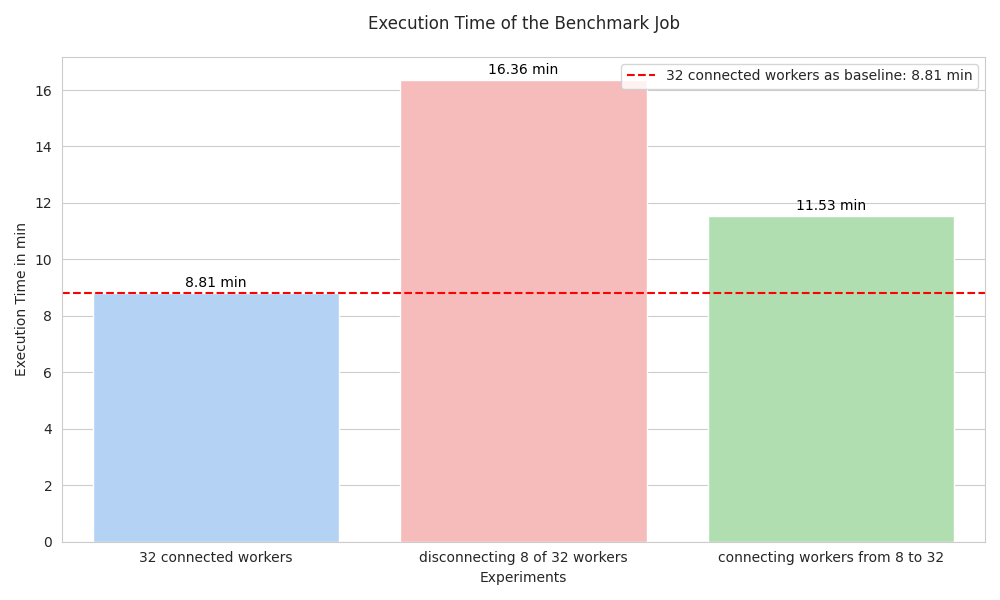
\includegraphics[width=0.95\textwidth]{gfx/figures/Evaluation_B.png}
    \caption{WebCrowd Execution Time in Dynamic Environment}
    \label{fig:evaluation:experiment-B}
\end{figure}
~\\
In experiment 1, the WebCrowd platform successfully demonstrated reliable task redistribution when workers are disconnecting during the computation of a task. The implemented timeout mechanism effectively rescheduled all 8 aborted tasks distributed to the 8 manually disconnected workers. The system maintained consistent progress despite losing up 25\% of the initial worker pool, though with a expected increases of the total computation time to 16 minutes and 21.6 seconds.

During experiment 2, the WebCrowd platform successfully integrated new workers as they joined, with each additional worker immediately receiving and computing tasks from the current batch after they successful initialized the corresponding WebAssembly environment. Since this experiment started with only 25\% of the amount of workers compared to the baseline experiment, it was expected that the total computation time is slower than the baseline. Corresponding, the total execution time of this experiment was 11 minutes and 31.8 seconds. 
\\~\\
Bouth experiments demonstrated that the WebCrowd platform can maintain operation continuity despite significant worker pool fluctuations. This validates WebCrowd's implementation for dynamic worker participation and confirms, that it is suitability for real-world volunteer computing scenarios where the availability of a worker device is not guaranteed.

\section{Heterogeneous Viability}
\label{sec:evaluation:heterogen}
\textbf{Does WebCrowd support a diverse range of client devices without issues?}
The third research question examines WebCrowd's capability to effectively support diverse client devices as workers, therfore also addressing a critical requirement for volunteer computing platforms. As the pool of potential worker devices in a real-world environment is expected to be diverse in hardware, software and operating systems \cite{intro:diverseDevices}, the following experiemnt is used to evaluate whether WebCrowd can successfully with a heterogeneous group of participating workers.

\subsection{Experimental Setup}
To evaluate the platform's support for heterogeneous devices, a diverse set of computing devices was assembled to participate simultaneously in the benchmark job through the WebCrowd platform. The following four devices represent different hardware architectures (ARM and x86), various operating systems (iOS, Windows, and Linux), and also different browser environments (Apple Safari 18.1 \cite{evaluation:safari}, Mozilla Firefox 132.0 \cite{background:firefox}, and Microsoft Edge 131.0.0.0 \cite{evaluation:edge}):
\begin{itemize}
    \item One smartphone as specified in \autoref{app:system:phone}
    \item One laptop as specified in \autoref{app:system:mymachine}, executing 3 worker tabs in parallel
    \item One \acs{PC} as specified in \autoref{app:system:mymachine}, executing 3 worker tabs in parallel
    \item One tablet as specified in \autoref{app:system:tablet}
\end{itemize}
All of these devices where found in one hoeshold to demonstrate the easy accessibility to a potential performance gain of a computational intensive job by leveraging the WebCrowd platform.

\subsection{Expectations}
It is expected that the bechmark job is successfully computed and that all participating workers are able to compute their scheduled tasks, regardless of the heterogeneous pool of connected devices. Furthermore, this set of devices - representing a single household - is expected to achieve a significant performance improvement compared to the baseline execution time of the natively computed Mandelbrot visualization on the server.  

\subsection{Results}
The Mandelbrot visualization job was again successfully computed and all participating workers were able to compute the tasks that have been distributed to them. Therfore, this experiment demonstrated WebCrowd's support for heterogeneous devices as workers. All devices successfully connected to the platform, initialized their WebAssembly environments, and computed their assigned tasks without any occuring issues. The WebSocket connections remained stable and the WebWorker-WebAssembly environment was effortlessly established across all corresponding browsers, which already came preinstalled to every used device. \autoref{fig:evaluation:experiment-C} displays the total computaion time of this experiment compared to the basline computation time of the native server environment measured in \autoref{sec:evaluation:computation}.
\begin{figure}[htbp]
    \centering
    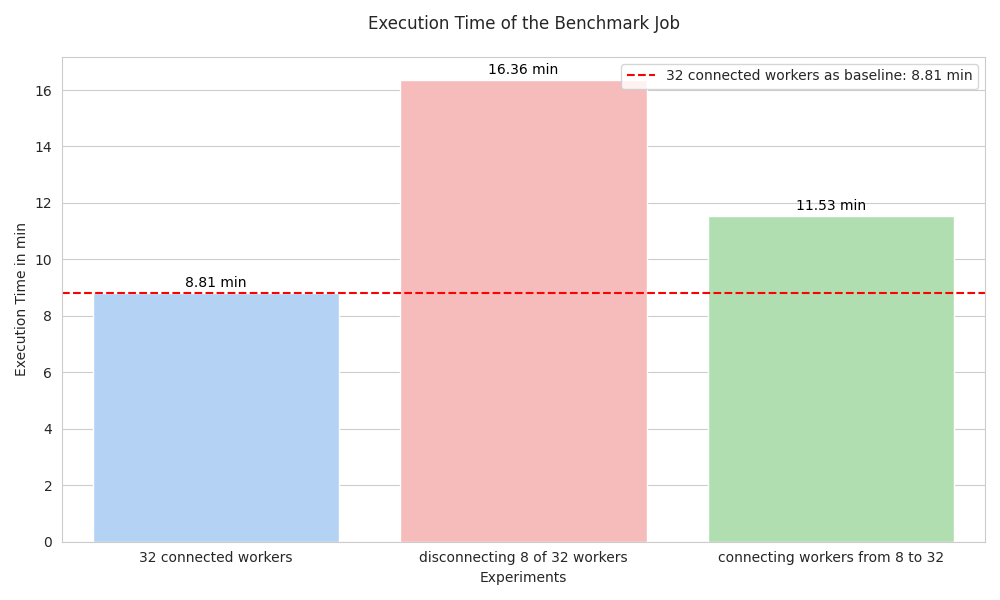
\includegraphics[width=0.95\textwidth]{gfx/figures/Evaluation_B.png}
    \caption{TODO}
    \label{fig:evaluation:experiment-C}
\end{figure}
~\\
blabla zu performace vergleich
\\~\\
The implemented web interface of the client page adapted appropriately to all different screen sizes and resolutions, providing a consistent user experience across all devices. Additionally, the WebWorker implementation effectively prevented any freezing effects of the the \ac{UI} during the computation of tasks on all tested browsers. Therfore, the web application maintained responsiv throughout the experiment and provided the monitoring of each worker, as intended.
\\~\\
These results validate WebCrowd's capability to support heterogeneous devices effectively. The platform successfully leveraged WebAssembly's platform independence to enable consistent computation across different architectures, while the web-based approach provided a uniform and easy-to-use application, accessible to any device with a modern browser. This confirms that WebCrowd achieves its design goal to ...

\section{Comparison of WebAssembly Environments}
\label{sec:evaluation:languages}